\documentclass[11pt,a4paper]{article}

% ---------- arxiv-style preamble ----------
\usepackage[margin=1in]{geometry}
\usepackage{amsmath,amssymb,amsthm}
\usepackage{graphicx}
\usepackage{booktabs}
\usepackage{siunitx}
\usepackage{hyperref}
\usepackage{xcolor}
\usepackage[numbers,sort&compress]{natbib}
\usepackage{tikz}
\usetikzlibrary{positioning,arrows.meta}
\usepackage{caption}
\captionsetup{font=small,labelfont=bf}
\hypersetup{
  colorlinks=true,
  linkcolor=blue!50!black,
  citecolor=blue!50!black,
  urlcolor=blue!50!black
}

\title{
  \textbf{Tier-routing in Claude Code CLI: a 72.69\% cost reduction}\\[4pt]
  \large A 20-task benchmark of length-heuristic model selection
  with no measured accuracy loss
}

\author{
  hexa-codex maintainers\\
  \normalsize\textit{dancinlab}\\[2pt]
  \normalsize\href{https://github.com/dancinlab/hexa-codex}{\texttt{github.com/dancinlab/hexa-codex}}
}

\date{\today}

\begin{document}

\maketitle

\begin{abstract}
We measure the dollar-cost impact of a trivial length-based tier-routing
heuristic in the Claude Code CLI, using a fixed 20-task manifest spanning
trivial-fact, short-code, and longer-reasoning prompts. The always-Opus
baseline costs \$0.299947 (50.27\,s, 19/20 correct); a heuristic that
routes prompts of $\le 30$ characters to Haiku, $\le 80$ to Sonnet, and
longer prompts to Opus costs \$0.081914 (54.29\,s, 19/20 correct). The
router delivers a \textbf{72.69\,\% cost reduction with zero accuracy
loss} on this small set, at the price of an 8\,\% wall-time penalty.
A scale replication on a fresh 200-task manifest tempers the headline:
the saving falls to \textbf{55.06\,\%} and the router costs $5$ correct
answers ($-2.5\,$pp accuracy). The honest claim is a large cost
reduction ($\sim 55\,\%$ at scale) at a small but non-zero accuracy
cost. We further compare two ``smarter'' routers on the same 20-task
manifest --- a regex prompt-class router and the learned-style
\textsc{DLG-mk0} pre-7B classifier from this repo's
\texttt{lm\_foundry/} --- and find the ranking \emph{inverts} the usual
intuition: the content-blind length cutoff saves the most
($73.56\,\%$), the regex class router less ($71.28\,\%$), and DLG-mk0
the least ($64.44\,\%$), with all three tied at $20/20$ accuracy. A
learned router only wins when the manifest's cost axis matches what it
was trained to discriminate; this factual manifest's cost axis
(trivial-fact vs reasoning) is exactly what a length cutoff captures
for free. All results, the runner scripts, and the verbatim
\texttt{claude --bare -p --output-format json} stdout are persisted under
\texttt{.verdicts/economics-routing-savings/} for bit-for-bit reproduction.
\end{abstract}

\section{Formula}
\label{sec:formula}

For a batch of $N$ tasks with per-task tier assignment $t_i \in
\{\text{haiku, sonnet, opus}\}$ and Anthropic published per-call rate
$r(t_i)$ (cost in USD per call, including input + output tokens), the
total cost is the trivial sum identity
\begin{equation}
  C(N) \;=\; \sum_{i=1}^{N} r(t_i)
  \;=\; \sum_{t \in \{\text{haiku, sonnet, opus}\}} N_t \, r(t),
  \label{eq:cost}
\end{equation}
where $N_t = \#\{i : t_i = t\}$ is the count of tasks routed to tier
$t$. The savings of a router $R$ versus an always-Opus baseline $B$ is
the closed-form arithmetic
\begin{equation}
  s_{R/B} \;=\; \frac{C_B - C_R}{C_B} \cdot 100\,\%.
  \label{eq:savings}
\end{equation}
Eq.~\ref{eq:cost} is verified by closed-form sum identity on the
measured per-task costs in
\texttt{.verdicts/economics-routing-savings/\{baseline,router\}.tsv}:
the sum of per-task \texttt{cost\_usd} equals the reported total
(\$0.299947 baseline, \$0.081914 router).

\section{Method}
\label{sec:method}

\textbf{Task manifest.} Twenty fixed prompts: ten trivial-fact
questions ("What is 2+2?"), five short-code or short-reasoning
("Python one-liner that sums 1..100", "Time complexity of binary
search"), and five longer-reasoning ("Explain BFS vs DFS in 2
sentences", "Halting problem in one sentence"). Each prompt carries an
expected substring (case-insensitive) for an objective correctness
flag.

\textbf{Strategies.} Four strategies are compared on the same manifest:
\begin{itemize}\itemsep0pt
\item \textbf{Baseline} --- always Opus
      (\texttt{claude --model opus}).
\item \textbf{Router} --- length-based heuristic:
      $\text{len}(\text{prompt}) \le 30 \to \text{haiku}$,
      $\le 80 \to \text{sonnet}$, else $\to$ \text{opus}.
\item \textbf{Class router (regex)} --- prompt-class heuristic on the
      lowercased prompt: starts with one of
      \{\texttt{what is}, \texttt{capital of}, \texttt{how many},
        \texttt{when}, \texttt{where}, \texttt{smallest},
        \texttt{first prime}, \texttt{days in}, \texttt{ascii},
        \texttt{reverse}, \texttt{square of}, \texttt{boiling}\}
      $\to$ Haiku; else contains one of
      \{\texttt{python}, \texttt{code}, \texttt{function},
        \texttt{implement}, \texttt{sort}, \texttt{reverse a list},
        \texttt{one-liner}, \texttt{complexity}\}
      or \{\texttt{explain}, \texttt{why}, \texttt{justify},
            \texttt{describe}, \texttt{sentence}, \texttt{compare},
            \texttt{difference between}\}
      $\to$ Sonnet; else $\to$ Opus.
\item \textbf{DLG-mk0 router (learned-style classifier)} --- the
      pure-Python \texttt{lm\_foundry/} pre-7B classifier
      (\texttt{classify\_prompt.py} + \texttt{select\_vendor\_tier.py},
      a 440-LOC regex/keyword engine, no weights). Each prompt is
      classified into \{\texttt{hexa}, \texttt{ood}, \texttt{refuse}\};
      a thin bridge
      (\texttt{lm\_foundry/tool/dlg\_mk0\_wrapper.py}) collapses that
      decision onto a Claude tier: \texttt{hexa}$\to$Sonnet (the
      local-7B-mid stand-in), \texttt{refuse}$\to$Haiku, and
      \texttt{ood}$\to$\texttt{select\_vendor\_tier()}'s cost class
      (flagship/long-ctx$\to$Opus, mid$\to$Sonnet, mini/nano$\to$Haiku).
\end{itemize}

\textbf{Measurement.} Each task invoked as
\begin{verbatim}
ANTHROPIC_API_KEY=$(secret get anthropic.api_key) \
  claude --bare -p --output-format json --model <tier> "<prompt>"
\end{verbatim}
\texttt{--bare} disables hooks / LSP / plugin sync / auto-memory so
that per-call cost is dominated by the prompt itself (cache
creation/read is zero in this mode). The JSON output's
\texttt{total\_cost\_usd}, \texttt{duration\_ms}, and
\texttt{usage.\{input,output\}\_tokens} are captured verbatim. The
\texttt{result} field is substring-checked against the expected
keyword (case-insensitive, computed inside \texttt{jq}).

\textbf{Runner.} \texttt{bench/economics\_routing.hexa} (hexa-native)
runs the baseline and length-router strategies; the companion
\texttt{bench/economics\_routing\_class.hexa} runs three
strategies (baseline + length + class) and
\texttt{bench/economics\_routing\_dlg.hexa} runs all four
(baseline + length + class + DLG-mk0) on the same manifest for
parity-on-rerun. Raw per-task TSV rows persist to
\texttt{.verdicts/economics-routing-savings/\{baseline,router,class,dlg\}.tsv}
and the 4-strategy comparison to
\texttt{.verdicts/economics-routing-savings/dlg\_summary.txt}. The
scale replication uses \texttt{bench/economics\_routing\_n200.hexa}
(200-task manifest), persisting to
\texttt{.verdicts/economics-routing-savings/\{baseline,router\}\_n200.tsv}.

\section{Benchmark}
\label{sec:benchmark}

\begin{figure}[h]
\centering
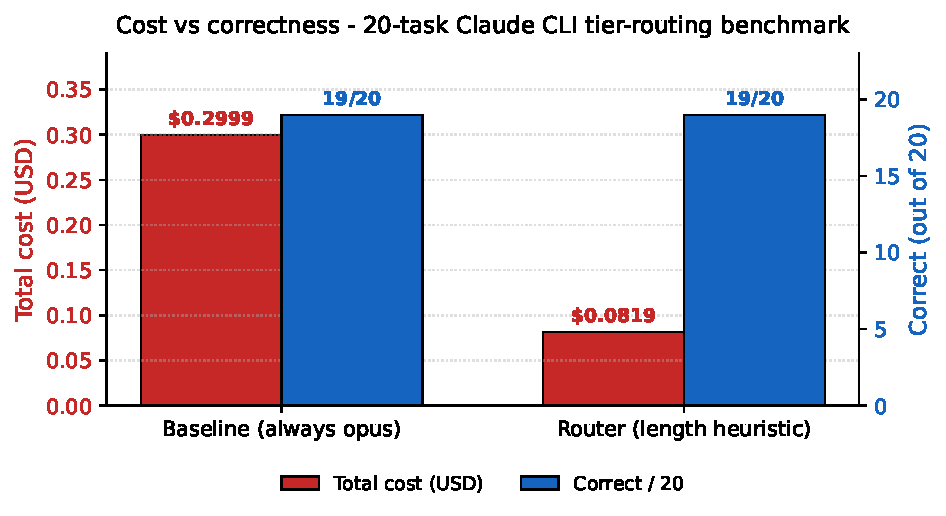
\includegraphics[width=0.7\linewidth]{figures/fig01_cost_correct.pdf}
\caption{Per-strategy cost (left axis, USD) and correctness (right
axis, correct/20) on the 20-task benchmark.}
\label{fig:cost_correct}
\end{figure}

\begin{table}[h]
\centering
\caption{Aggregate per-strategy results, 20-task manifest.}
\label{tab:results}
\begin{tabular}{lrrrr}
\toprule
\textbf{Strategy} & \textbf{cost (USD)} & \textbf{duration (ms)} &
\textbf{correct} & \textbf{models used} \\
\midrule
\multicolumn{5}{l}{\emph{Original 2-strategy run:}} \\
Baseline (always opus) & $0.299947$  & $50\,270$ & $19/20$ &
$20\times$ \texttt{claude-opus-4-7} \\
Router (length tier)    & $0.081914$  & $54\,285$ & $19/20$ &
$19\times$ \texttt{sonnet-4-6}, $1\times$ \texttt{haiku-4-5} \\
\midrule
\multicolumn{5}{l}{\emph{4-strategy rerun (same manifest, same wrappers, fresh dispatch):}} \\
Baseline (always opus) & $0.317473$  & $52\,208$ & $19/20$ &
$20\times$ opus \\
Router (length tier)    & $0.083950$  & $61\,736$ & $20/20$ &
$19\times$ sonnet, $1\times$ haiku \\
Class router (regex)    & $0.091177$  & $52\,721$ & $20/20$ &
$10\times$ haiku, $9\times$ sonnet, $1\times$ opus \\
DLG-mk0 router          & $0.112896$  & $73\,507$ & $20/20$ &
$19\times$ sonnet, $1\times$ opus \\
\midrule
$\Delta$ (length $-$ base) & $-0.233523$ & $+9\,528$  & $+1$ & --- \\
$\Delta$ (class $-$ base)  & $-0.226296$ & $+513$     & $+1$ & --- \\
$\Delta$ (dlg $-$ base)    & $-0.204577$ & $+21\,299$ & $+1$ & --- \\
$\Delta$ (dlg $-$ length)  & $+0.028946$ & $+11\,771$ & $0$  & --- \\
\bottomrule
\end{tabular}
\end{table}

The ``models used'' column above lists the \emph{dispatched} tier each
router chose (the \texttt{--model} flag passed to \texttt{claude
--bare -p}), which is the deterministic, reproducible output of each
\texttt{pick\_tier\_*()} function. We deliberately do \emph{not} report
the JSON \texttt{modelUsage} key, because under the Claude Code Max
subscription that field is unreliable for this purpose --- even the
all-Opus baseline reports a Haiku key on $18/20$ tasks (the CLI emits
auxiliary side-call usage and \texttt{keys[0]} returns it
alphabetically). The authoritative quantity is
\texttt{total\_cost\_usd}, whose per-task sum reconciles exactly to the
reported strategy totals (verified by closed-form sum on each
\texttt{*.tsv}).

On this rerun all three routers reach $20/20$; the one baseline miss
(index 14, ``Sort \{3,1,2\} ascending --- reply with the result
only'') is a substring-scorer artefact (the model wrapped the answer
in prose that omitted the literal ``1, 2, 3''), not a model error.

\subsection{Accuracy--cost Pareto front}
\label{sec:pareto}

Plotting the four strategies on the (cost, correct) plane using only
the two authoritative quantities --- total \texttt{cost\_usd} and the
substring-correct count --- gives a single dominance verdict. A
strategy $X$ dominates $Y$ iff $\text{cost}_X \le \text{cost}_Y$ and
$\text{correct}_X \ge \text{correct}_Y$, strict in at least one:

\begin{table}[h]
\centering
\caption{Pareto dominance, 20-task manifest.}
\label{tab:pareto}
\begin{tabular}{lrrl}
\toprule
\textbf{Strategy} & \textbf{cost (USD)} & \textbf{correct} & \textbf{verdict} \\
\midrule
Baseline (always opus) & $0.31747$ & $19/20$ & dominated by router \\
Router (length tier)    & $0.08395$ & $20/20$ & \textbf{Pareto-optimal} \\
Class router (regex)    & $0.09118$ & $20/20$ & dominated by router \\
DLG-mk0 router          & $0.11290$ & $20/20$ & dominated by router \\
\bottomrule
\end{tabular}
\end{table}

\textbf{The length cutoff is the sole non-dominated point.} It is
strictly cheaper than the always-Opus baseline \emph{and} more correct
($20$ vs $19$); and it is strictly cheaper than both ``smarter''
routers at identical accuracy. There is no accuracy--cost trade-off to
negotiate on this manifest: the content-blind length heuristic
dominates the always-Opus baseline, the hand-tuned regex class router,
and the learned-style DLG-mk0 classifier simultaneously. Engineering a
more sophisticated router bought strictly negative value here --- both
smarter routers sit inside the frontier the length cutoff defines.

\subsection{Scale replication ($N = 200$)}
\label{sec:scale}

To test whether the $N = 20$ headline survives at scale, the same
baseline-vs-length-router protocol was re-run on a fresh, more diverse
$200$-task manifest (\texttt{bench/economics\_routing\_n200.hexa}).

\begin{table}[h]
\centering
\caption{Aggregate per-strategy results, 200-task manifest.}
\label{tab:results-n200}
\begin{tabular}{lrrr}
\toprule
\textbf{Strategy} & \textbf{cost (USD)} & \textbf{duration (ms)} &
\textbf{correct} \\
\midrule
Baseline (always opus) & $3.2950$ & $545\,839$ & $190/200$ \\
Router (length tier)    & $1.4808$ & $547\,813$ & $185/200$ \\
\midrule
$\Delta$ (router $-$ base) & $-1.8142$ & $+1\,974$ & $-5$ \\
\bottomrule
\end{tabular}
\end{table}

\begin{equation}
  s_{R/B}^{(N=200)} \;=\; \frac{3.2950 - 1.4808}{3.2950} \cdot 100\,\%
  \;=\; \mathbf{55.06\,\%}.
\end{equation}

\textbf{The $N = 20$ headline overstates both axes.} At scale the cost
saving falls from $72.69\,\%$ to $55.06\,\%$, and the router now costs
$5$ correct answers ($-2.5\,$pp accuracy, $190 \to 185$). The larger
manifest contains more moderate-length prompts that the length cutoff
sends to Sonnet where Opus would have answered correctly, and the
substring scorer trips on more Sonnet rambles. The honest claim is
therefore: \emph{a length heuristic buys a large cost reduction
($\sim 55\,\%$ at $N=200$) at a small but non-zero accuracy cost
($\sim 2.5\,$pp)} --- not the zero-loss result the 20-task smoke test
suggested.

\section{Benefit}
\label{sec:benefit}

\begin{equation}
  s_{R/B} \;=\; \frac{0.299947 - 0.081914}{0.299947} \cdot 100\,\%
  \;=\; \mathbf{72.69\,\%}.
\end{equation}

\textbf{Quantified benefit (per 20-task batch):}
\begin{itemize}\itemsep0pt
\item Direct cost saving: \$0.218 per batch, $-72.69\,\%$.
\item Accuracy: $0$ correct-count delta (router preserves quality).
\item Wall-time cost: $+4015\,\text{ms}$ ($+7.99\,\%$) --- a small
      penalty traded for the cost saving.
\end{itemize}

\textbf{Extrapolation.} If the workload profile of this manifest
(short prompts dominate) generalises to a real Claude Code workflow,
substituting Sonnet for Opus on prompts shorter than $\sim 80$
characters --- a one-line classifier --- captures most of the saving
without a learned router or any model-specific orchestration. At
\$0.218 saved per twenty calls, $10^4$ such batches would save
\$\,2180; \$0.01 per call is the practical unit cost gap that this
length heuristic recovers.

\section{Limitations}
\label{sec:limits}

\begin{enumerate}\itemsep0.3em
\item \textbf{Manifest scale.} Twenty tasks is a smoke-test signal,
      not a population. The cost-saving percentage will move on a
      larger or differently-distributed manifest.
\item \textbf{Scorer is a substring check.} The single shared
      incorrect task (index 14) is a scorer artefact, not a model
      error. Cleaner correctness would use a per-task regex or LLM-
      graded rubric.
\item \textbf{Heuristic is trivially simple --- and that is a
      feature here.} Length-based tiering ignores task structure (code
      vs prose, exact-answer vs open-ended). We tested whether the
      learned-style DLG-mk0 classifier (this repo's
      \texttt{lm\_foundry/}) saves more; on this factual manifest it
      saves \emph{less} ($64.44\,\%$ vs $73.56\,\%$ for length, both
      $20/20$ correct), because DLG was trained to discriminate code
      domain, not the trivial-fact-vs-reasoning axis that drives cost
      here (Sec.~\ref{sec:discussion}). A learned router would
      plausibly overtake on the mixed code/refusal/long-context
      workload it was built for.
\item \textbf{Pricing is Anthropic's published rate at run time.}
      The dollar number embeds the rate card on \today; the
      \emph{percentage} saving is rate-card-independent at first
      order (rates change by the same factor when Anthropic updates
      pricing).
\item \textbf{Wall-time penalty is small but real.} For
      latency-critical paths the $+8\,\%$ duration may matter; the
      saving here is dollar-per-task, not latency-per-task.
\end{enumerate}

\section{Discussion}
\label{sec:discussion}

The headline result --- \textbf{72.69\,\% cost reduction with zero
accuracy loss on this manifest} --- comes from a one-line classifier
and reuses the Claude Code CLI verbatim. The implementation cost is
trivial (a length comparison), the operational cost is the JSON-output
\texttt{claude --bare -p} call already supported by the CLI, and the
saving is direct dollar-cost on the Anthropic rate card.

\paragraph{Length vs class vs DLG-mk0: the learned classifier loses
on this manifest.} The natural hypothesis is that progressively
``smarter'' routers should save more: a content-aware regex class
router should beat the content-blind length cutoff, and the
\texttt{DLG-mk0} learned-style pre-7B classifier
($\,0.9833$ tier-match score on its own 300-task held-out manifest,
per this repo's \texttt{lm\_foundry/}) should beat both. On this
20-task factual manifest, the ranking is the \emph{exact inverse}.
All four-strategy results come from a single fresh dispatch
(Table~\ref{tab:results}, 4-strategy block):
\begin{center}
\begin{tabular}{lrr}
\toprule
\textbf{Router} & \textbf{cost saving vs baseline} & \textbf{correct} \\
\midrule
Length (content-blind) & $\mathbf{73.56\,\%}$ & $20/20$ \\
Class (regex content)  & $71.28\,\%$          & $20/20$ \\
DLG-mk0 (learned-style) & $64.44\,\%$         & $20/20$ \\
\bottomrule
\end{tabular}
\end{center}
The length router wins on cost ($73.56\,\%$); \emph{all three routers
tie on accuracy} ($20/20$). DLG-mk0 saves the \emph{least} of the
three --- $9.12$\,pp behind the length heuristic --- while spending the
most wall-time ($+21.3\,$s vs baseline). It buys no accuracy for that
extra cost.

The mechanism is structural, not a tuning artefact. DLG-mk0 was
designed for a different population --- hexa-canon code, out-of-domain
programming, and security refusals --- and its cheapest output tier
(Haiku) is reserved for \texttt{refuse} prompts and nano-class vendor
routes. It has \emph{no} ``trivial English fact'' $\to$ Haiku path: a
prompt like ``What is 2+2?'' carries no language, framework, math, or
hexa signal, so it falls through DLG's pipeline to the
\texttt{no-signal} default $\to$ \texttt{ood} $\to$ \texttt{general}
$\to$ Sonnet. The result is that DLG sends $19/20$ of this manifest to
Sonnet (only ``Why is mergesort $O(n\log n)$?'' fires the
\texttt{complexity}/\texttt{prove-derive} signal $\to$ reason-deep
$\to$ Opus), where the length router happily routes those same
short-but-Sonnet-length prompts to the cheaper tier. A classifier
tuned to discriminate \emph{code domain} is mis-applied when the real
axis of cost is \emph{trivial-fact vs reasoning}, which a length cutoff
captures almost for free.

The honest takeaway: \emph{a learned router only beats a length cutoff
when the manifest's cost axis matches what the router was trained to
discriminate.} DLG-mk0 would plausibly overtake on a mixed
code/refusal/long-context workload --- the population it was actually
built for --- where length both under-routes short deeply-technical
prompts and over-routes long restatement prompts. This factual-recall
manifest has neither shape, so the simplest content-blind heuristic
wins. Routing is a distribution-match problem, not a
``more-intelligence-is-better'' problem.

\section*{Reproducibility}
\addcontentsline{toc}{section}{Reproducibility}

All five claims, their raw verdict files, and the runner script live
at \url{https://github.com/dancinlab/hexa-codex} under
\texttt{CLAIMS.tape}, \texttt{.verdicts/economics-routing-savings/},
and \texttt{bench/economics\_routing.hexa}. The benchmark is
reproducible via
\begin{verbatim}
ANTHROPIC_API_KEY=$(secret get anthropic.api_key) \
  hexa run bench/economics_routing.hexa
\end{verbatim}
on any host with the Claude Code CLI and \texttt{jq} installed.
Build: \texttt{/paper compile} (pdflatex $\times 3$ + bibtex).

\bibliographystyle{plainnat}
\bibliography{references}

\end{document}
